\documentclass{article}

\usepackage[spanish]{babel}
\usepackage[utf8]{inputenc} % Idioma, tildes y ñ. Hace falta guardar como UTF-8

\usepackage{algorithm}	%Pseudocódigo
\usepackage{algorithmic}

\usepackage{amsthm} %Demostraciones

\usepackage{amsmath} %Alinear ecuaciones

\usepackage[none]{hyphenat}	%No partir palabras al final de la linea

\usepackage{graphicx}	%Imágenes

\usepackage{float}	%Respetar orden de imágenes y algoritmos

\begin{document}
\sloppy
\title{Algoritmos de Aproximaci\'on}

\author{Daniel Valverde Menasalvas}

\maketitle

\newtheorem{thr}{Teorema}[section]
%%%%%%%%%%%%%%%%%%%%%%%%%%%%%%%%Introducción
\section{Introducción}
\label{sec:introduction}
Hay muchos problemas NP-completos que son demasiado importantes como para abandonarlos simplemente por no poder obtener una soluci\'on \'optima. Como poco, tendremos tres posibles enfoques para este tipo de problemas: 
\begin{enumerate}
	\item Utilizar un algoritmo de coste exponencial en casos con pocos datos de entrada.
	\item Aislar casos especiales que se puedan resolver con coste polin\'omico.
	\item Utilizar algoritmos que encuentren soluciones cercanas a la \'optima con coste polin\'omico.
\end{enumerate}

Un algoritmo que devuelve soluciones cercanas a la \'optima se llama algoritmo de aproximaci\'on. En este trabajo se expondrán algoritmos de aproximaci\'on con coste polin\'omico para varios problemas NP-completos.\\

\subsection{Radio de comportamiento para algoritmos de aproximaci\'on}
Decimos que un algoritmo tiene, para un problema, un \textbf{radio de comportamiento} $\rho(n)$ si, para cualquier entrada de tamaño $n$, el coste $C$ de la soluci\'on producida por el algoritmo y el coste $C*$
 de la soluci\'on \'optima cumplen: 
\[
	\max(\frac{C}{C^{*}}, \frac{C^{*}}{C}) \leq \rho(n)
\]


Esta definici\'on sirve para problemas de maximizaci\'on y minimizaci\'on. Un radio de comportamiento de $1$ indica una soluci\'on \'optima y uno muy grande indica una mala aproximaci\'on. A los algoritmos que consiguen un radio de aproximaci\'on de $\rho(n)$ los llamamos \textbf{$\rho(n)-$algoritmos de aproximaci\'on}.\\

Un \textbf{esquema de aproximaci\'on} para un problema de optimizaci\'on es un algoritmo de aproximaci\'on que toma como input un valor $\epsilon > 0$ de forma que, dado un $\epsilon$, el esquema es un $(1 + \epsilon)-$algoritmo de aproximaci\'on. Un esquema de aproximaci\'on es un \textbf{algoritmo de aproximaci\'on en tiempo polin\'omico} si dado un $\epsilon > 0$, el esquema tiene coste polin\'omico en el tamaño de los datos de entrada.\\

Decimos que un esquema de aproximaci\'on es un \textbf{esquema de aproximaci\'on completamente polin\'omico} si es polin\'omico en $1/\epsilon$ y en el tamaño de los datos de entrada. Un ejemplo ser\'ia $O((1/\epsilon)^2n^3)$. De esta manera, si somos menos exigentes con la precisi\'on de la solución del algoritmo (aumentamos $\epsilon$) veremos una disminuci\'on en el tiempo de ejecuci\'on.

%%%%%%%%%%%%%%%%%%%%%%%%%%%%Vertex-cover%%%%%%%%%%%%%%%%%%%%%%%%%%%%%%%%%%%%%%%%
\section{El problema del recubrimiento por v\'ertices (vertex-cover)}\label{sec:vertexCover}
El recubrimiento por v\'ertices de un grafo no dirigido $G = (V,E)$ es un subconjunto $V' \subseteq V$ tal que si $(u, v)$ es una arista de $G$, entonces $ u \in V' \vee v \in V'$. El tamaño de $V'$ es el n\'umero de v\'ertices que contiene. \\

El problema del recubrimiento por v\'ertices es encontrar un recubrimiento de tamaño m\'inimo (\textbf{recubrimiento \'optimo por vertices}) en un grafo no dirigido. Aunque es dif\'icil encontrar una soluci\'on \'optima a este problema, no lo es tanto encontrar una soluci\'on aproximada. El siguiente algoritmo toma un grafo no dirigido $G$ y devuelve un recubrimiento por v\'ertices cuyo tamaño es, a lo sumo, el doble del \'optimo $(\rho(n) = 2)$.\\


\begin{algorithm}[H]
\caption{APPROX-VERTEX-COVER($G$)}
\begin{algorithmic}[1]
\STATE $C\gets \emptyset $
\STATE $E' \gets G[E]$
\WHILE{$E'\neq\emptyset$}%\Comment{si lo quieres explicar}
\STATE sea $(u,v)$ una arista arbitraria de $E$
\STATE $C \gets C \cup \{u,v\}$
\STATE eliminar de $E'$ toda arista incidente en $u$ o $v$
\ENDWHILE
\RETURN {$C$}
\end{algorithmic}
\end{algorithm}


Si usamos una lista de adyacencia para representar $E'$, el tiempo de ejecuci\'on del algoritmo está en $O(V + E)$.\\

\begin{figure}[H]
  \centering
    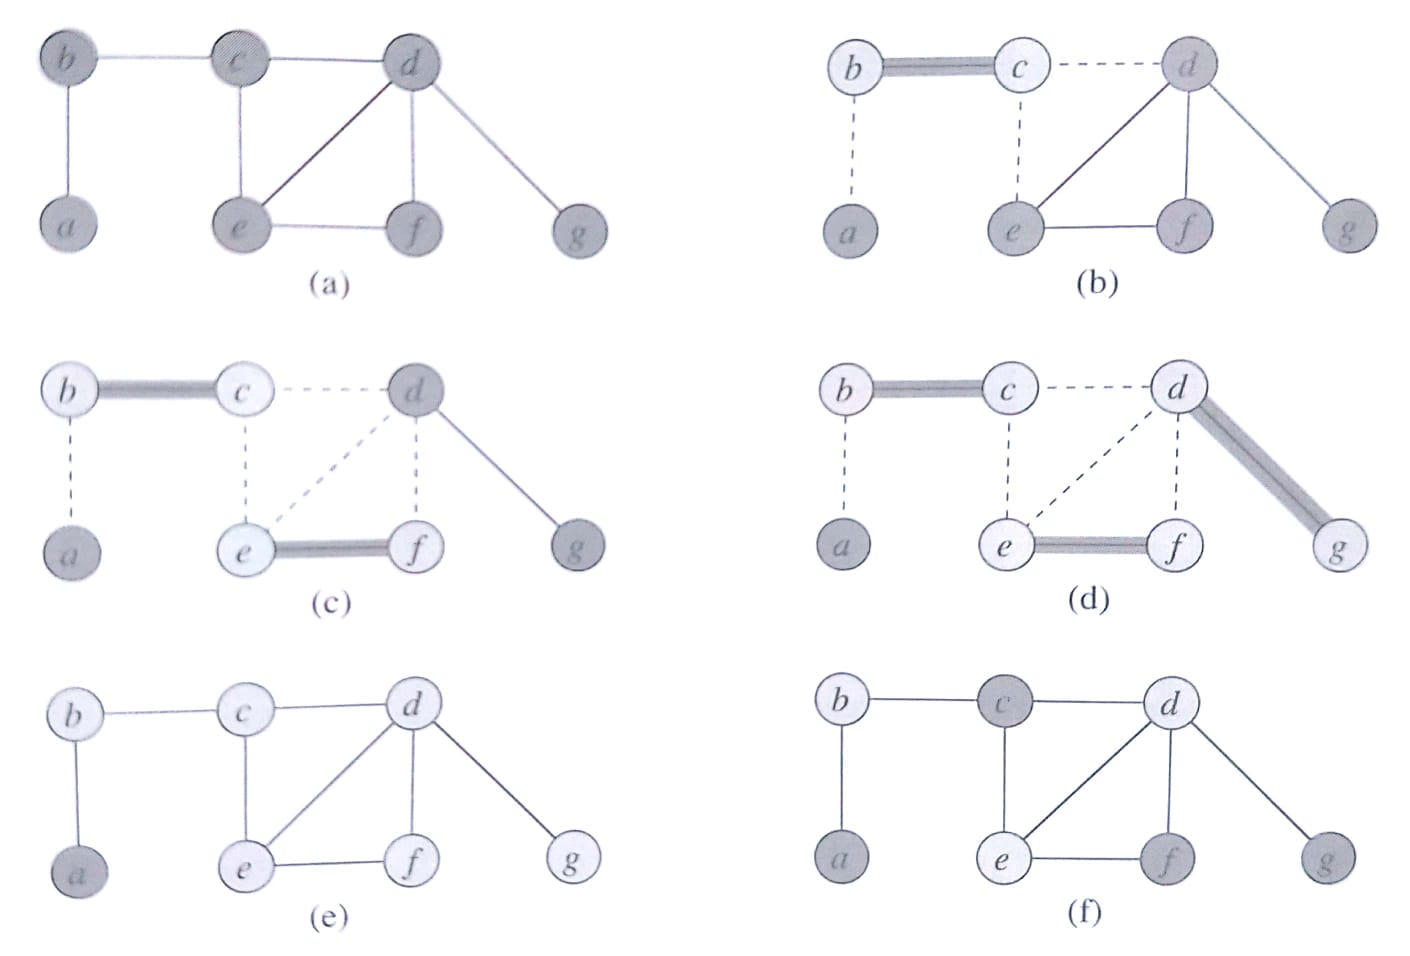
\includegraphics[width=0.7\textwidth]{vertex-cover}
  \caption{Ejemplo gráfico del algoritmo APPROX-VERTEX-COVER}
\end{figure}

\begin{thr}
APPROX-VERTEX-COVER es un 2-algoritmo de aproximaci\'on en tiempo polin\'omico.
\end{thr}
\begin{proof}[Demostración]
Ya sabemos que el algoritmo es polinómico. El conjunto de vértices $C$ devuelto por el algoritmo es un recubrimiento por vértices ya que el bucle del algoritmo no termina hasta que recubre todas sus aristas con algún vértice de $C$.\\ 
Para ver que $C$ es, como mucho, el doble de grande que el recubrimiento óptimo $C*$, llamaremos $A$ al conjunto de aristas que el algoritmo coge en la linea $4$. No hay dos aristas en $A$ que compartan un vértice incidente ya que, al escoger una arista para $A$, el algoritmo elimina de $E'$ todas las aristas que inciden en cualquiera de los dos vértices de la arista escogida. Por lo que no hay dos aristas en $A$ que estén cubiertas por el mismo vértice de $C^{*}$, lo que nos da un límite inferior para el tamaño de la solución óptima:\\
$|C^{*}| \geq |A|$\\
Además, cada iteración del bucle elige una arista para $A$ que no incida en ninguno de los vértices de $C$, lo que nos permite expresar el tamaño de $C$ como:\\
$|C| = 2|A|$\\
Juntando las dos ecuaciones obtenidas obtenemos el resultado buscado:\\
$|C| = 2|A| \leq 2|C^{*}|$ 	
\end{proof}

%%%%%%%%%%Problema del viajante%%%%%%%%%%
\section{El problema del viajante}
Dado un grafo $G = (V,E)$ no dirigido y valorado positivamente, el problema del viajante se basa en encontrar un ciclo hamiltoniano de $G$ con coste mínimo. Este problema es NP-completo incluso si la función de costes cumple la desigualdad triangular.\\

Decimos que la función de costes del grafo, $c(u,v)$, satisface la \textbf{desigualdad triangular} si para cualesquiera $u, v, w \in V$, $c(u,w) \leq c(u,v) + c(v,w)$. Esta propiedad se satisface numerosas veces de manera natural, por ejemplo, si el grafo está compuesto por puntos del plano y $c$ es la distancia entre ellos. A continuación se expone un algoritmo para el problema del viajante cumpliendo la desigualdad triangular.

\begin{algorithm}[H]
\caption{APPROX-TSP-TOUR($G,c$)}
\begin{algorithmic}[1]
\STATE elegimos un vértice $r \in V[G]$ para ser raíz
\STATE generamos un árbol recubridor mínimo $T$ para $G$ desde $r$ usando el algoritmo de Prim
\STATE sea $L$ la lista de vértices de $T$ en pre-orden
\RETURN {el ciclo hamiltoniano $H$ que visita los vértices en el orden $L$}
\end{algorithmic}
\end{algorithm}

\begin{figure}[H]
  \centering
    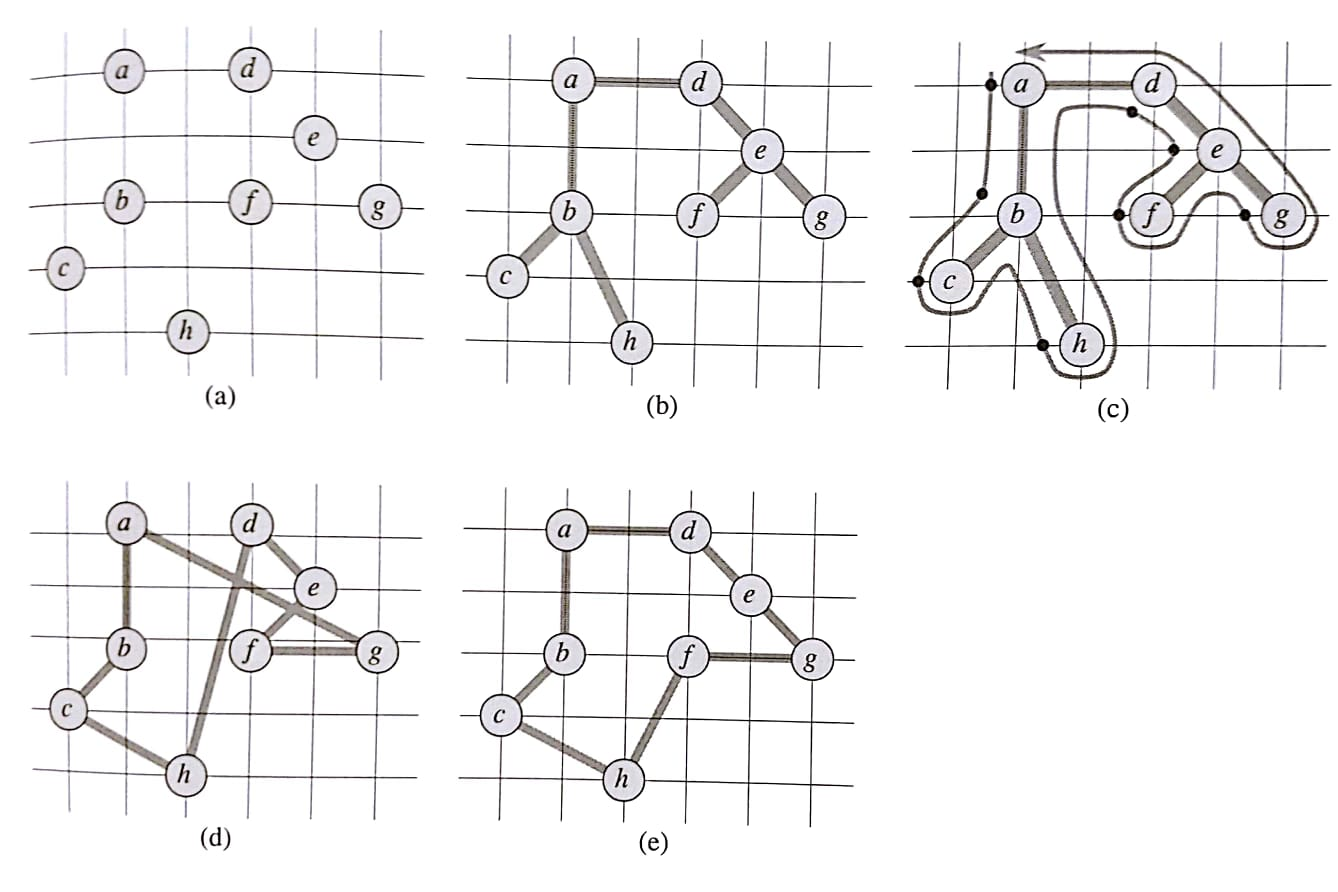
\includegraphics[width=0.7\textwidth]{TSP}
  \caption{Ejemplo gráfico del algoritmo APPROX-TSP-TOUR}
\end{figure}

\begin{thr}
APPROX-TSP-TOUR es un 2-algoritmo de aproximaci\'on en tiempo polin\'omico del problema del viajante con la desigualdad triangular.
\end{thr}
\begin{proof}[Demostración]
Ya hemos visto que APPROX-TSP-TOUR es un algoritmo polinómico. \\
Sea $H^{*}$ una solución óptima del problema. Al quitar una arista de un ciclo hamiltoniano obtenemos un árbol recubridor, y el coste de cada arista es no negativo. Por lo tanto, el coste del árbol recubridor mínimo obtenido en el algoritmo nos da una cota inferior del coste de la solución óptima:\\
$c(T) \leq c(H^{*})$\\
Llamaremos \textbf{recorrido completo} de un árbol $T$ a una lista donde aparecen los vértices cuando son visitados por primera vez y también cuando volvemos a pasar por ellos tras visitar un subarbol. Llamemos $W$ al recorrido completo de $T$. El recorrido completo de nuestro ejemplo sería:\\
$a, b, c, b, h, b, a, d, e, f, e, g, e, d, a$\\
Como el recorrido completo pasa por cada arista de $T$ exactamente dos veces, tenemos(extendiendo la definición de coste $c$ de manera natural para soportar conjuntos en los que haya aristas repetidas)\\
$c(W) = 2c(T)$\\
Juntando las dos ecuaciones vista hasta ahora tenemos\\
$c(W) \leq 2c(H^{*})$\\
por lo que el coste de $W$ es, como mucho, el coste de $H^{*}$.\\
Por desgracia, $W$ no es generalmente un ciclo hamiltoniano ya que puede visitar cada vértice más de una vez. Sin embargo, usando la desigualdad triangular, podemos omitir una visita a cualquier vértice de $W$ sin aumentar su coste(eliminar la visita al vértice $v$ de $W$ que esta entre las visitas a $u$ y a $w$ significa ir directamente de $u$ a $w$). Repitiendo esta operación, podemos eliminar todas las visitas a vértices en $W$ a excepción de la primera visita a cada vértice. En nuestro ejemplo quedaría:\\
$a, b, c, h, d, e, f, g$\\
Este orden es el obtenido al recorrer con preorden el árbol $T$. Sea $H$ el ciclo correspondiente a este listado de vértices. Es un ciclo hamiltoniano pues cada vértice se recorre exactamente una vez y, de hecho, es el ciclo que devuelve nuestro algoritmo. Como $H$  es obtenido eliminando vértices de $W$, tenemos el resultado buscado:\\
$c(H) \leq c(W) \leq 2c(H^{*})$
\end{proof}
	
Si quitamos la condición de que $c$ cumpla la desigualdad triangular, no se pueden encontrar buenas aproximaciones de este problema a no ser que $P = NP$. Es posible demostrar que, si $P \neq NP$, dado cualquier $\rho(n) \geq 1$, no hay ningún $\rho(n)$-algoritmo de aproximación con tiempo polinómico para el problema general del viajante.

\section{El problema del conjunto de cobertura}
El problema del conjunto de cobertura es un problema de optimización que modela muchos problemas de selección de recursos, entre ellos el del recubrimiento por vértices. Sin embargo, el algoritmo mostrado en la sección \ref{sec:vertexCover} no es aplicable aquí, por lo que intentaremos otros enfoques con un radio de aproximación logarítmico.\\

Una instancia $(X,F)$ del problema del conjunto de cobertura consiste en un conjunto finito $X$ y una familia $F$ de subconjuntos de $X$, tal que cada elemento de $X$ pertenece a, al menos, un subconjunto en $F$. El problema se trata de encontrar un subconjunto $C \subseteq F$ con el menor número de elementos posible que recubra $X$.\\

El problema del conjunto de cobertura es una abstracción de diversos problemas típicos de combinatoria. Un ejemplo sencillo sería el de tener un conjunto $X$ de habilidades necesarias para realizar un trabajo y una serie de personas, cada una con alguna de esas habilidades. El problema consistiría en obtener un equipo de personas con el menor número de integrantes posible tal que, para cada habilidad, haya al menos una persona en el equipo que la tenga.\\

Propondremos un algoritmo voraz para resolver el problema. Este consiste en coger, en cada etapa del problema, el subconjunto $S$ que cubra el mayor número de elementos no cubiertos. El algoritmo es el siguiente:\\

\begin{algorithm}[H]
\caption{GREEDY-SET-COVER($X,F$)}
\begin{algorithmic}[1]
\STATE $U \gets X$
\STATE $C \gets \emptyset$
\WHILE{$U \neq \emptyset$}%\Comment{si lo quieres explicar}
\STATE elegir un $S$ que maximice $|S \cap U|$
\STATE $U \gets U - S$
\STATE $C \gets C \cup \{S\}$
\ENDWHILE
\RETURN {$C$}
\end{algorithmic}
\end{algorithm}

\begin{figure}[H]
  \centering
    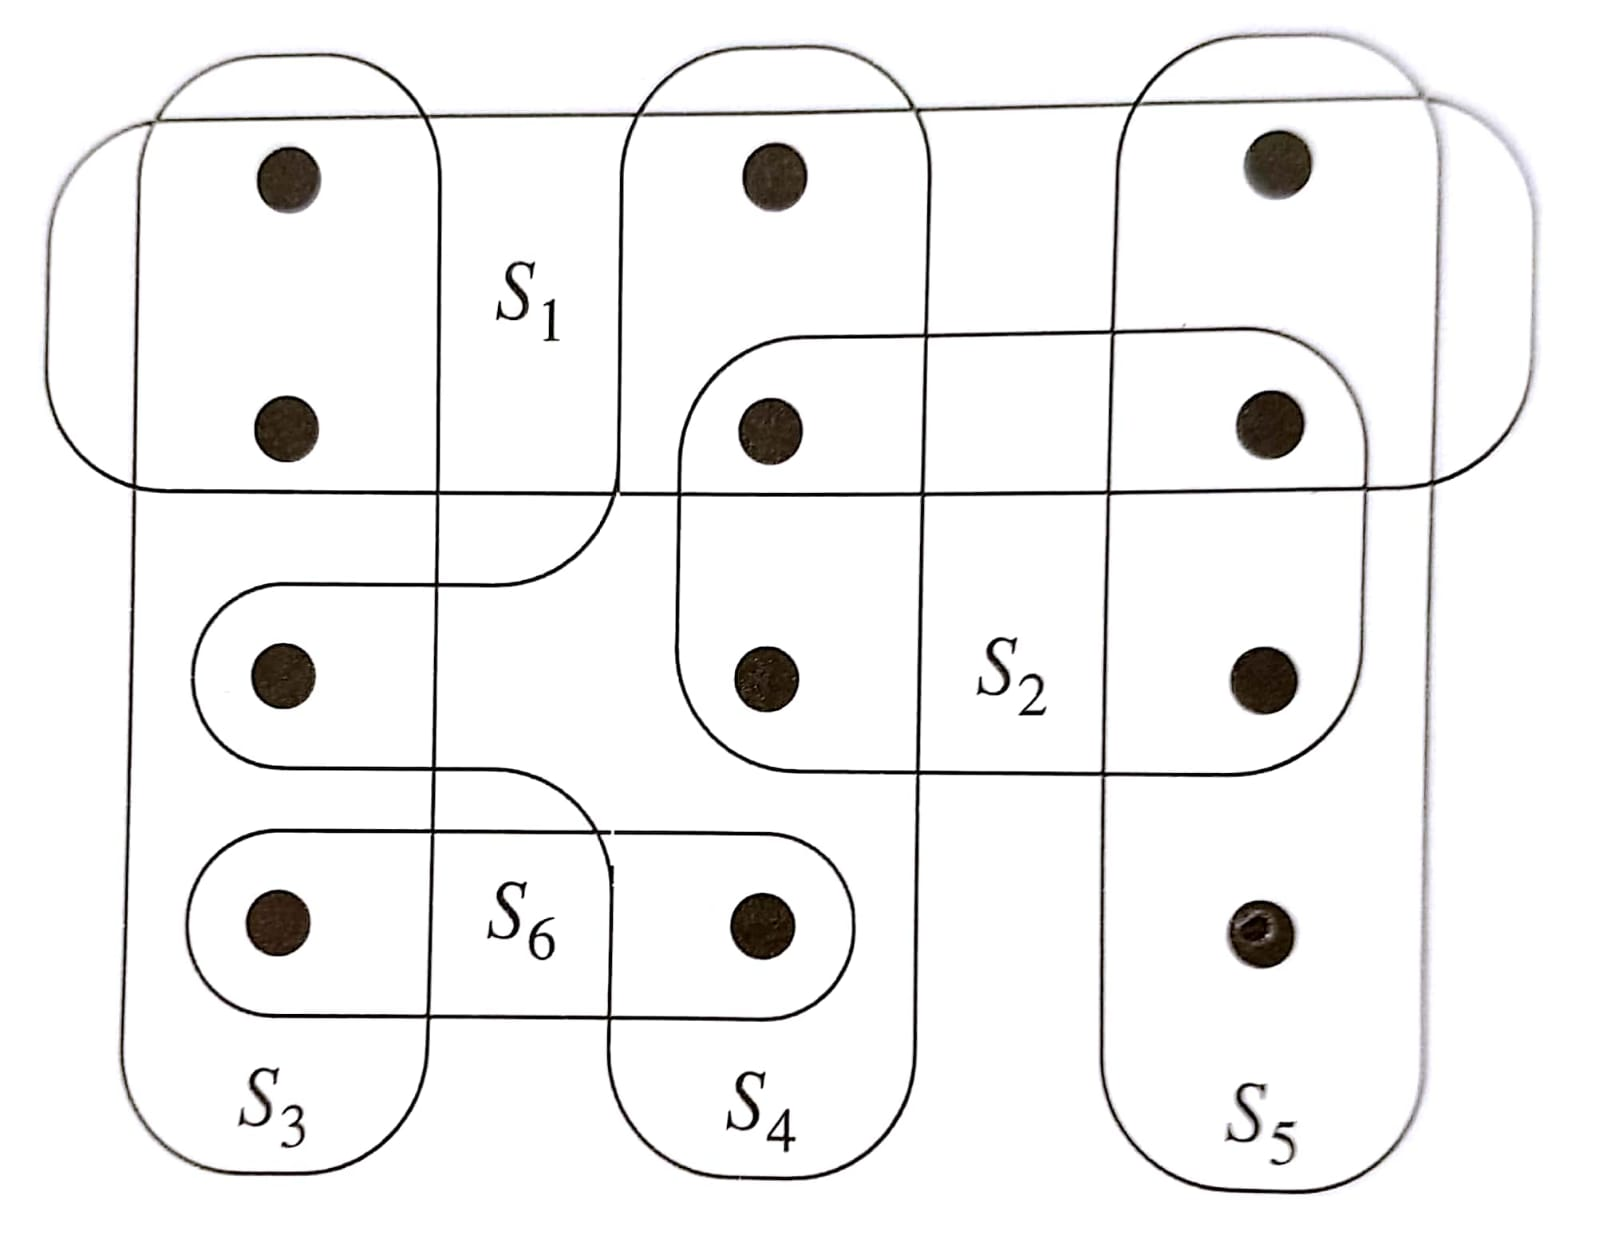
\includegraphics[width=0.7\textwidth]{set-cover}
  \caption{Ejemplo gráfico del problema del conjunto de cobertura. 
El algoritmo GREEDY-SET-COVER elegiría los conjuntos: $S_1, S_4, S_5, S_3$ (podría cambiarse $S_3$ por $S_6$, esta elección depende de la implementación del algoritmo).}
\end{figure}

El bucle de las líneas 3-6 se ejecuta, a lo sumo, $\min(|X|,|F|)$ veces y el cuerpo del bucle puede ser implementado en $O(|X||F|)$. Por lo tanto, se puede hacer una implementación simple de este algoritmo de orden $O(|X||F|\min(|X|,|F|))$. Aunque omitiremos la prueba debido a su extensión, este algoritmo es un $\rho(n)$-algoritmo de aproximación en tiempo polinómico, donde $\rho(n) = H(max{|S|:S \in F})$, siendo $H(d) = \sum_{i=1}^{d}1/i$. Los detalles de esta demostración se pueden encontrar en \cite[pág 1120]{cormen}.\\

Al ser $\frac{1}{x}$ una función monótona decreciente tenemos
\begin{gather*}
	\sum_{k=2}^{n}\frac{1}{k} \leq \int_{1}^{n}\frac{dx}{x} = \ln n \\ 	
	\sum_{k=1}^{n}\frac{1}{k} \leq  \ln n + 1
\end{gather*}
 Consecuencia directa de esto último es que el algoritmo es también un $(ln|X| + 1)$-algoritmo de aproximación en tiempo polinómico.

\section{Aleatorización y programación lineal}
En esta sección estudiaremos dos técnicas útiles para diseñar algoritmos de aproximación: aleatorización y programación lineal.

\subsection{Un algoritmo de aproximación aleatorizado para la satisfacibilidad de MAX-3-CNF}
Una \textbf{3-forma normal conjuntiva (3-CNF)} es una expresión booleana formada por cláusulas unidas por AND de 3 literales unidos por OR. Un ejemplo sería $(x_1 \vee x_3 \vee \neg x_2) \wedge (x_3 \vee x_2 \vee x_4) \wedge(\neg x_1 \vee \neg x_3 \vee \neg x_4)$. El problema de la satisfacibilidad de 3-CNF trata de determinar la satisfacibilidad de una fórmula puesta en 3-CNF, y es un problema NP-completo.\\

Si una fórmula 3-CNF no es satisfactible, puede que queramos saber `cómo de cerca' esta de serlo, es decir, cuál es el número máximo de cláusulas que se pueden satisfacer a la vez. Este problema es denominado \textbf{la satisfacibilidad de MAX-3-CNF}. El objetivo es encontrar una asignación para cada variable que maximice el número de cláusulas que se evalúan a 1.

\begin{thr}
Dada una instancia de la satisfacibilidad de MAX-3-CNF con $n$ variables y $m$ cláusulas, el algoritmo aleatorizado que, independientemente, pone cada variable a 1 con probabilidad 1/2 y a 0 con probabilidad 1/2 es un (8/7)-algoritmo de aproximación aleatorizado.
\end{thr}
\begin{proof}[Demostración]
Consideremos la variable aleatoria $Y_{i} = I\{$ la cláusula $i$ evalúa $1$ $\}$ de forma que $Y_{i} = 1$ si alguno de los literales que la componen evalúa $1$. Como no hay dos literales iguales en una misma cláusula, ni tampoco uno y su negado, el valor de cada uno de los literales de una cláusula es independiente. Para que una cláusula evalué $0$, sus tres literales deben evaluar $0$, por lo que $P\{$cláusula $i$ evalua $0\} = (1/2)^{3} \rightarrow P\{$cláusula $i$ evalua $1\} = 1 - 1/8 = 7/8$. Sea $Y = Y_{1} + Y_{2} + ... + Y_{m}$. Entonces
\begin{gather*}
	E[Y] = E[\sum_{i=1}^{m}Y_{i}] = \sum_{i=1}^{m}E[Y_{i}] = \sum_{i=1}^{m}7/8 = 7m/8
\end{gather*}
Claramente, m es un límite superior del número de cláusulas evaluando $1$, por lo tanto el radio de aproximación es, como mucho $m/(7m/8) = 8/7$.

\end{proof}

\subsection{Aproximando el recubrimiento por vértices valorados usando programación linear}
El \textbf{problema del mínimo recubrimiento por vértices valorados} es similar al problema del recubrimiento por vértices salvo que, en este caso, cada vértice tiene asociado un valor positivo, y buscamos un recubrimiento que tenga el menor valor posible. El valor de un recubrimiento es la suma de los valores de los vértices por los que está compuesto.\\

Si en este problema usamos el algoritmo de la sección \ref{sec:vertexCover} o uno aleatorizado obtendríamos soluciones con ratios de aproximación demasiado grandes. Sin embargo, podemos conseguir un límite inferior de la solución del problema usando programación lineal. Después `redondearemos' esta solución para obtener un recubrimiento por vértices.\\

Llamaremos $w(v)$ a la valoración del vértice $v$ y asociaremos una variable binaria $x(v)$ a cada vértice de $V$. Interpretaremos que $v$ forma parte de nuestro recubrimiento si y solo si $x(v) = 1$.  De esta manera podemos interpretar el problema del recubrimiento por vértices valorados como el siguiente problema de programación binaria:\\

minimizar	\begin{gather*}
\sum_{v \in V}w(v)x(v)
\end {gather*}
	
sujeto a
\begin{gather*}
	x(u) + x(v) \geq 1 \ \forall u, v \in V \\
	        x(v) \in \{0,1\} \ \forall v \in V
\end{gather*}
		
	

Este problema es NP-completo, sin embargo, podemos cambiar la condición de que $x(v) \in \{0,1\}$ por $0 \leq x(v) \leq 1$. De esta manera obtenemos el siguiente problema de programación lineal denominado \textbf{problema de programación lineal relajado}:\\

minimizar
\begin{gather*}
\sum_{v \in V}w(v)x(v)
\end{gather*}
	
sujeto a
\begin{gather*}
	x(u) + x(v) \geq 1 \ \forall v, u \in V \\
	        x(v) \leq 1 \  \forall v \in V \\
					x(v) \geq 0 \ \forall v \in V
\end{gather*}
		
		
			
Una solución factible del problema binario es también solución factible del problema lineal. De esta manera, una solución óptima del problema lineal es límite inferior de la solución del problema binario (es necesariamente menor o igual) y, por lo tanto, límite inferior del recubrimiento por vértices valorados. El algoritmo mostrado a continuación usa la solución de la relajación del problema linear para construir una solución aproximada al problema del mínimo recubrimiento por vértices valorados:\\

\begin{algorithm}[H]
\caption{APPROX-MIN-WEIGHT-VC($G,w$)}
\begin{algorithmic}[1]
\STATE $C \gets \emptyset$
\STATE Computar una solución $X$ para el problema de programación lineal
\FOR {each $v \in V$}%\Comment{si lo quieres explicar}
\IF {$X(v) \geq 1/2$}
\STATE $C \gets C \cup \{v\}$
\ENDIF
\ENDFOR
\RETURN {$C$}
\end{algorithmic}
\end{algorithm}

Este algoritmo genera un recubrimiento eligiendo los vértices a los que la solución $X$ del problema lineal había asignado valor 1/2 o más. A esto nos referíamos cuando decíamos que ´redondeábamos' la solución del problema de programación lineal.\\

\begin{thr}
APPROX-MIN-WEIGHT-VC es un 2-algoritmo de aproximación de tiempo polinómico para el problema del recubrimiento mínimo por vértices valorados
\end{thr}
\begin{proof}[Demostración]
Hay algoritmos que resuelven sistemas lineales en tiempo polinómico y el bucle for de las lineas $3-5$ también tiene coste polinómico por lo que el algoritmo es polinómico.\\
Sea $C^{*}$ una solución óptima del problema, y $z^{*}$ la solución óptima del problema de programación lineal. Como un recubrimiento por vértices óptimo es una solución factible del sistema lineal, $z^{*}$ debe ser un límite inferior de $w(C^{*})$, es decir, $z^{*} \leq w(C^{*})$.\\
Ahora veremos que si redondeamos los valores fraccionales de las variables $
\bar{x}(v)$, generamos un conjunto $C$ que es recubrimiento por vértices y satisface $w(C) \leq 2z^{*}$. Para ver que $C$ es un recubrimiento por vértices, consideramos una arista cualquiera $(u,v) \in E$. Sabemos que $x(u) + x(v) \geq 1$, lo que implica que por lo menos una de las variables $\bar{x}(u)$ y $\bar{x}(v)$ es al menos $1/2$. Por lo tanto, al menos uno de los vértices $u$ y $v$ está en el recubrimiento por vértices, por lo que cada arista está cubierta.\\
Ahora estudiaremos el coste del recubrimiento. Tenemos\\
	\[
	z^{*} = \sum_{v\in V}w(v)\bar{x}(v) \\
	\geq \sum_{v\in V:\bar{x}(v)\geq 1/2}w(v)\bar{x}(v) 
	\geq \sum_{v\in V:\bar{x}(v)\geq 1/2}w(v)\frac{1}{2} 
	\]
\[
	= \sum_{v\in C}w(v)\frac{1}{2} =\frac{1}{2}\sum_{v\in C}w(v) \\
	= \frac{1}{2}w(C)
\]

Lo que nos da $w(C) \leq 2z^{*} \leq 2w(C^{*})$ y el resultado buscado queda probado.

\end{proof}

\section{El problema de la suma de subconjuntos}
Dado un par $(S,t)$, donde $S$ es un conjunto de $n$ enteros positivos y $t$ es otro entero positivo, el problema de la suma de subconjuntos consiste en determinar si existe un subconjunto de S cuya suma sea exactamente t. El problema es NP-completo.\\

Este problema lleva asociado otro problema de optimización que consiste en encontrar un subconjunto de $S$ cuya suma sea lo mayor posible, sin llegar a ser mayor que $t$. Una aplicación práctica de este problema sería un camión con el que queremos transportar unas cajas de diferentes pesos de la forma más eficiente posible, es decir, llevando en cada viaje el máximo peso posible que pueda soportar el camión.

\subsection{Un algoritmo exacto de coste exponencial}
Antes de mostrar el algoritmo, son necesarias unas definiciones. La función MERGE-LISTS devuelve una lista formada por los integrantes de las dos listas que recibe como argumentos. Estos estarán ordenados y no se permitirán duplicados. La función tiene coste $O(|L|+|L'|)$ y se omitirá su pseudocódigo debido a su sencillez, aunque sí se incluirá su implementación en el código de C++. Definimos también el conjunto $S + x = \{ s + x : s \in S\}$.\\

A continuación se muestra un algoritmo que computa, con coste exponencial, todas las posibles sumas de subconjuntos de $S$ (al menos las que no excedan  $t$) y devuelve la que más se acerque a $t$ sin pasarse. \\

\begin{algorithm}[H]
\caption{EXACT-SUBSET-SUM($S,t$)}
\begin{algorithmic}[1]
\STATE $n \gets |S|$
\STATE $L_0 = \{0\} $
\FOR {$i \gets 1$ to $n$}%\Comment{si lo quieres explicar}
\STATE $L_i \gets MERGE-LISTS(L_{i-1}, L_{i-1} + x_i)$
\STATE Borramos de $L_i$ todo elemento mayor que $t$
\ENDFOR
\RETURN Mayor elemento en $L_n$
\end{algorithmic}
\end{algorithm}
  
\subsection{Un esquema de aproximación completamente polinómico}
A partir de la solución exponencial podremos crear un esquema de aproximación completamente polinómico para el problema de la suma de subconjuntos.\\

Para ello, simplificaremos las listas $L_i$ en cada iteración del bucle for. La simplificación se hará conforme a un parámetro $0 < \delta < 1$. Si $L$ es la lista inicial y $L'$ es la lista simplificada para cada elemento $y \in L$ existirá un $z \in L'$ tal que:
\[
\frac{y}{1 + \delta} \leq z \leq y
\]
El algoritmo de simplificación es lineal en el número de objetos de la lista L. Se expone a continuación un ejemplo: dado $\delta = 0.1$ y $L = \ <10, 11, 12 ,15, 20, 21, 22, 23, 24, 29>$, la lista simplificada es $L' = \ <10, 12, 15, 20, 23, 29>$.\\

Una vez definido el método de simplificación, podemos mostrar el algoritmo de aproximación para el problema de la suma de subconjuntos. Es posible demostrar que este algoritmo es un esquema de aproximación completamente polinómico para el problema dado, sin embargo, omitiremos su demostración debido a su extensión. Los detalles de esta se pueden encontrar en \cite[pág 1132]{cormen}.\\

\begin{algorithm}[H]
\begin{algorithmic}[1]
\STATE $m \gets |L|$
\STATE $L' \gets <y_1>$
\STATE $last \gets y_1$
\FOR {$i \gets 2$ to $m$}%\Comment{si lo quieres explicar}
\IF {$y_i > last(1 + \delta)$}
\STATE Añadir $y_i$ al final de $L'$
\COMMENT{$y_i \geq last$ ya que $L$ está ordenada}
\STATE $last \gets y_i$
\ENDIF
\ENDFOR
\RETURN $L'$
\end{algorithmic}
\caption{TRIM($L$,$\delta$)}
\end{algorithm}

\begin{algorithm}[H]
\begin{algorithmic}[1]
\STATE $n \gets |S|$
\STATE	 $L_0 = \{0\} $
\FOR {$i \gets 1$ to $n$}%\Comment{si lo quieres explicar}
\STATE $L_i \gets MERGE-LISTS(L_{i-1}, L_{i-1} + x_i)$
\STATE $L_i \gets TRIM(L_i, \epsilon/2n)$
\STATE Borramos de $L_i$ todo elemento mayor que $t$
\ENDFOR
\RETURN Mayor elemento en $L_n$
\end{algorithmic}
\caption{APPROX-SUBSET-SUM($S,t,\epsilon$)}
\end{algorithm}

\\

\begin{thebibliography}{x}
\bibitem{cormen} \textsc{Cormen,T.H.; Leiserson,C.E.; Rivest,R.L.; Stein,C.},
\textit{Introduction to Algorithms}
2ª ed. The Massachusetts Institute of Technology, 2001. 

\end{thebibliography}
\end{document}
